\chapter{Validaci\'on y Resultados}
\label{chap:resultados}

\section{validacion}
Dado que la salida del SGP4 ofrece las coordenadas en el sistema TEME, y que los datos provistos
por CODS est\'an publicados en el sistema TOD, hicimos un m\'odulo de transformaci\'on que validamos
utilizando el software STK.\\
Se detallan a continuaci\'on los resultados en ambos softwares y se verifica que las diferencias son peque\~nas, 
alcanzando m\'aximos del orden de cent\'imetros.\\

Salida ARxCODE.\\

\begin{tabular}{lcccccc}
2012-05-25 00:00& 6123.226358& -2799.6061073& 2030.22212402& 1.509737& -1.894738& -7.130677\\
2012-05-25 00:01& 6201.109925& -2907.4340358& 1598.47477776& 1.085502& -1.698287& -7.255920\\
2012-05-25 00:02& 6253.396906& -3003.2608146& 1160.11171533& 0.656815& -1.494839& -7.351125\\
2012-05-25 00:03& 6279.873805& -3086.6920159& 716.947643232& 0.225465& -1.285245& -7.415900\\
2012-05-25 00:04& 6280.434799& -3157.3849876& 270.816930972& -0.20674& -1.07038& -7.449981\\
2012-05-25 00:05& 6255.082153& -3215.0502978& -176.43422104& -0.63802& -0.85114& -7.453239
\end{tabular}

Salida STK.\\

\begin{tabular}{lcccccc}
25 May 2012 00:00& 6123.226382& -2799.605966& 2030.222245& 1.509738& -1.894738& -7.130677\\
25 May 2012 00:01& 6201.109963& -2907.433903& 1598.474875& 1.085502& -1.698287& -7.255921\\
25 May 2012 00:02& 6253.396954& -3003.260689& 1160.111787& 0.656816& -1.494840& -7.351126\\
25 May 2012 00:03& 6279.873859& -3086.691896& 716.947689&  0.225466& -1.285246& -7.415901\\
25 May 2012 00:04& 6280.434856& -3157.384873& 270.816951& -0.206748& -1.070381& -7.449982\\
25 May 2012 00:05& 6255.082210& -3215.050188& -176.434228& -0.638022& -0.851142& -7.453238
\end{tabular}

\section{Tendencia Anual 26/07/2011 - 26/07/2012}
\begin{figure}[!h]
\centering
  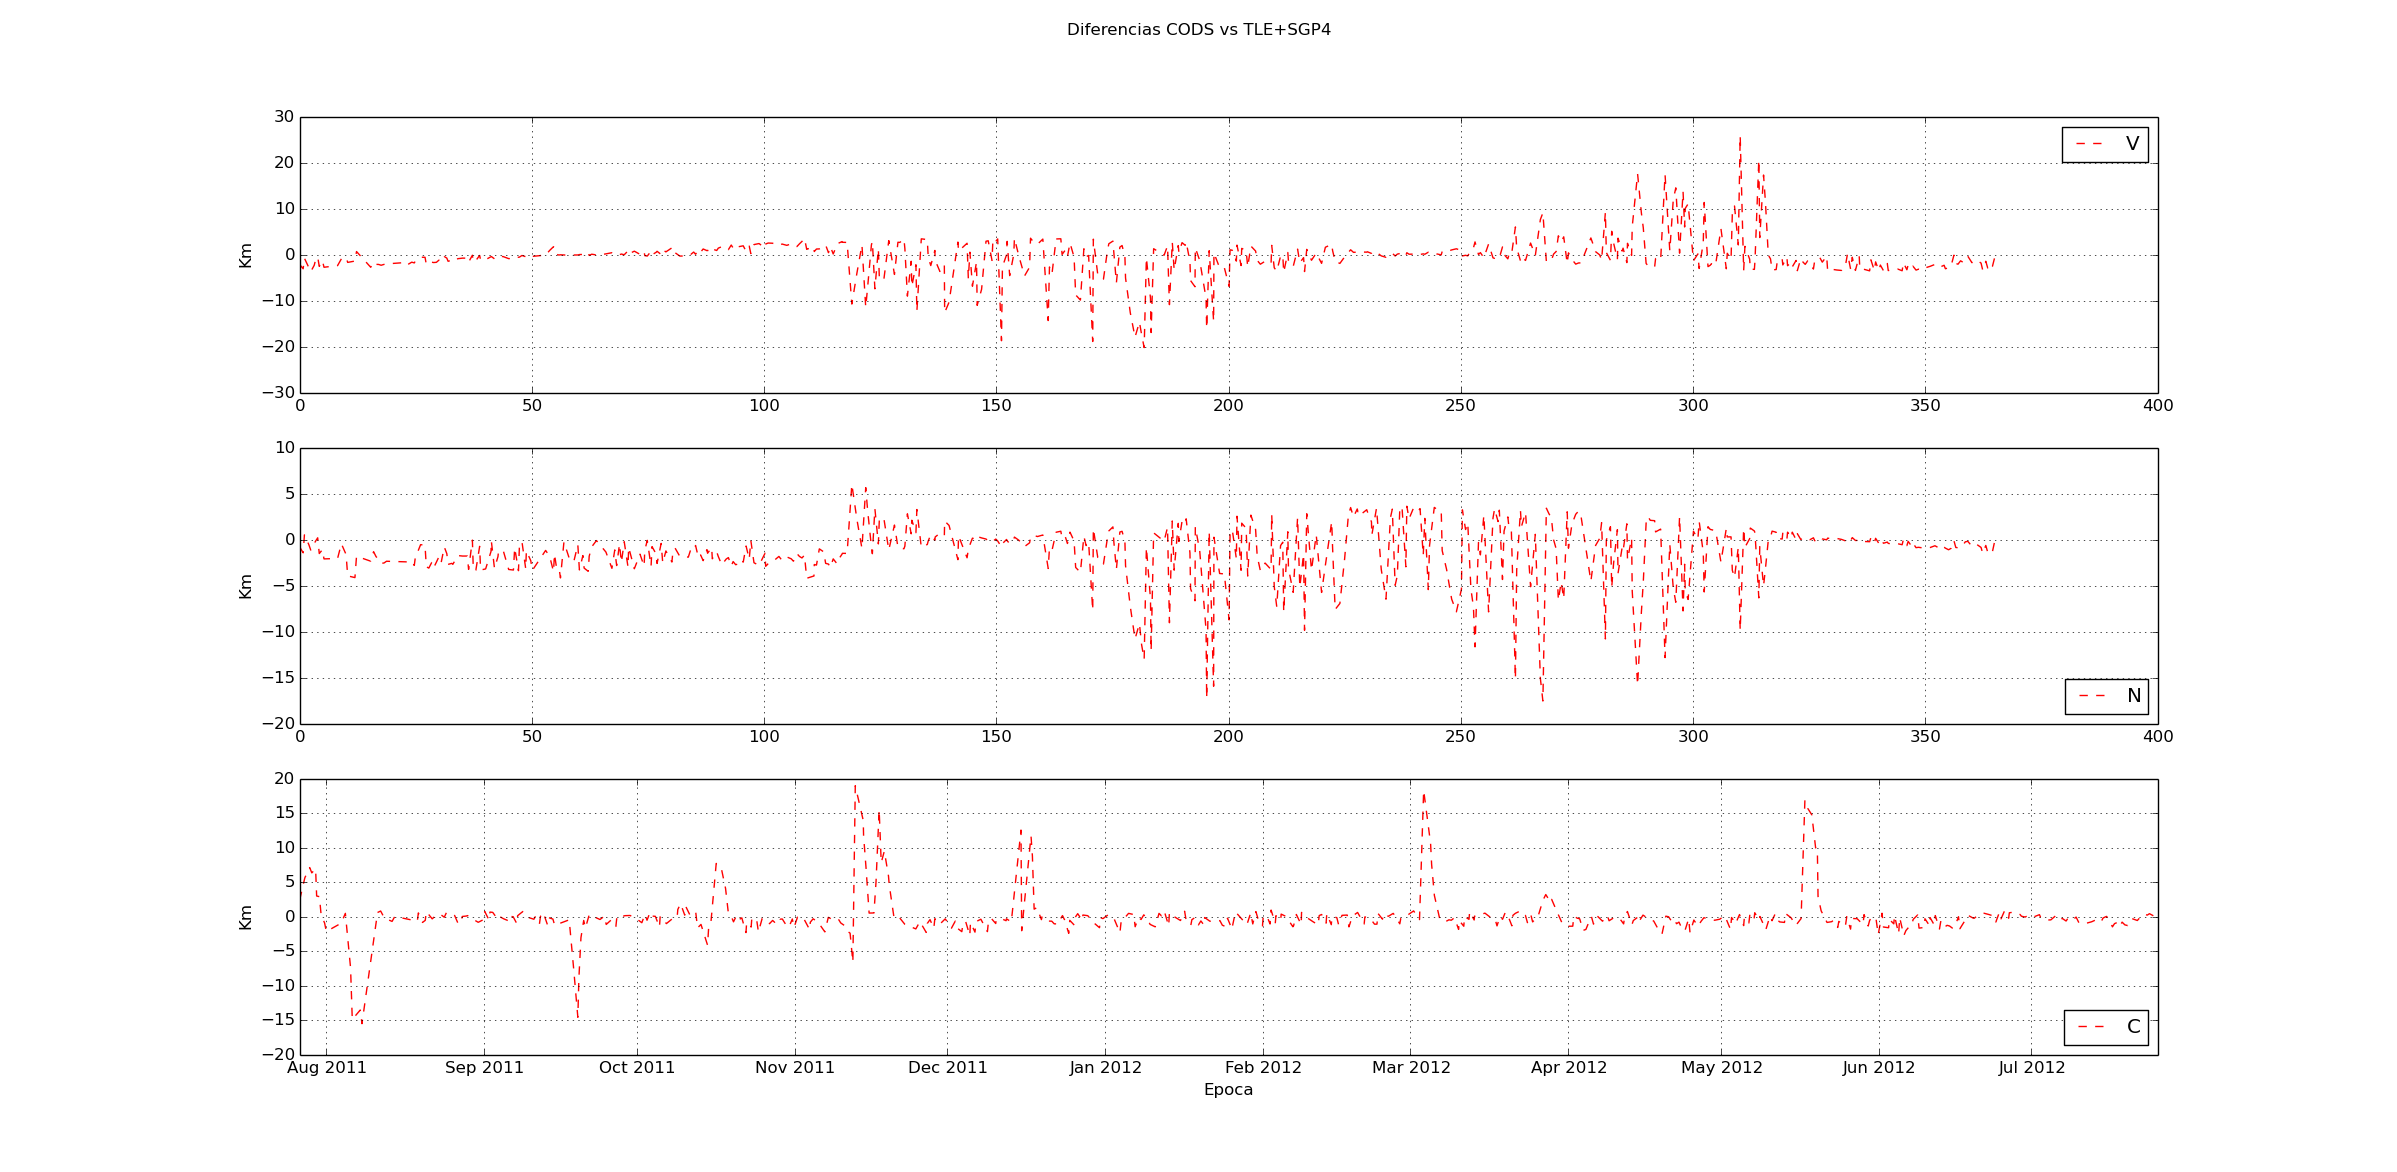
\includegraphics[width=\textwidth]{imagenes/sacDtendenciaAnualVNC}
\end{figure}
\begin{figure}[!h]
\centering
  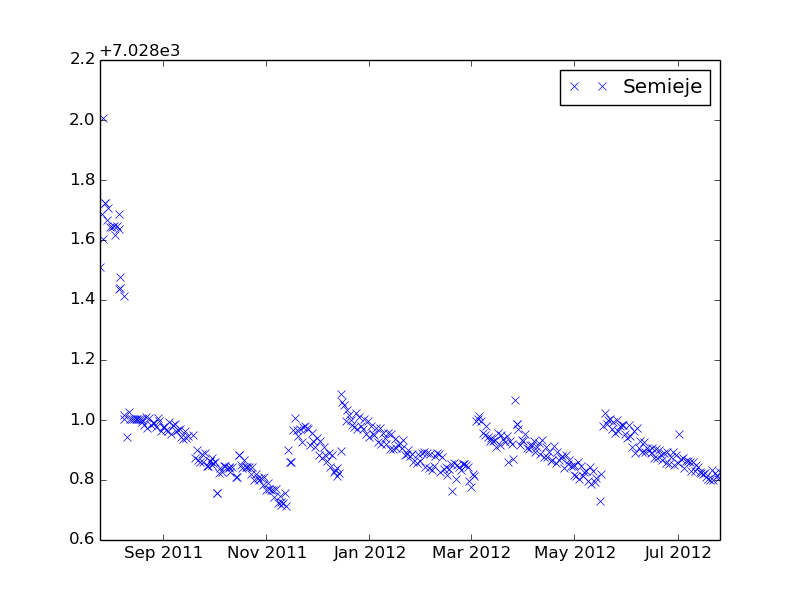
\includegraphics[width=0.7\textwidth]{imagenes/sacDtendSemi}
\end{figure}
\begin{figure}[!h]
\centering
  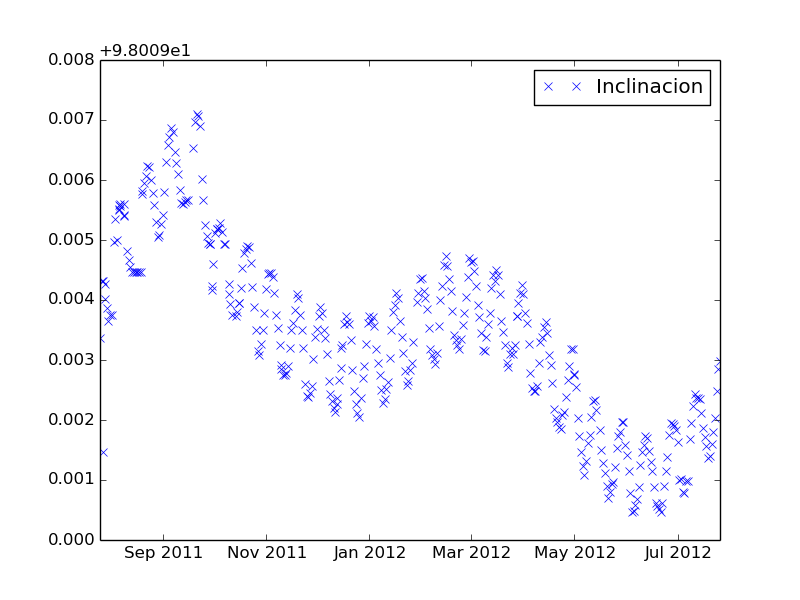
\includegraphics[width=0.7\textwidth]{imagenes/sacDtendInc}
\end{figure}


\section{AJUSTES 26/07/2011 - 26/07/2012}
\subsection{Lineal}
\begin{figure}[!h]
\centering
  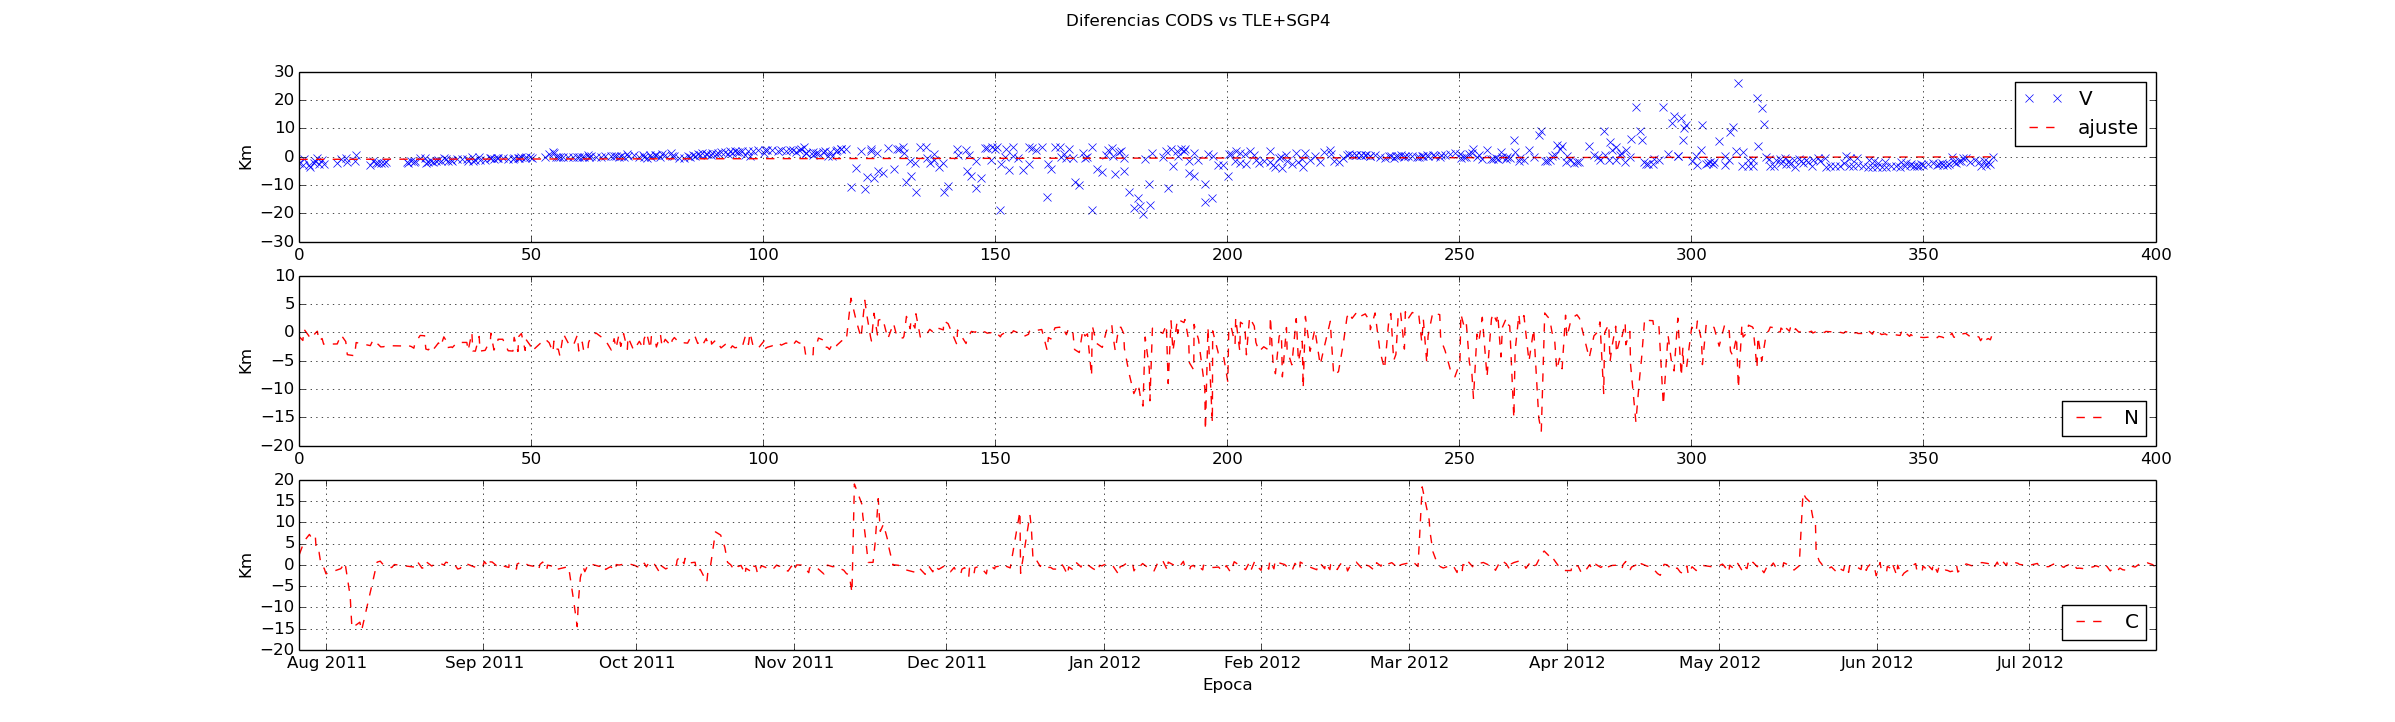
\includegraphics[width=\textwidth]{imagenes/sacDajusteG1}
\end{figure}
\begin{verbatim}
[-0.91541786  0.00237725]
[array([ 10308.58816238]), 2, array([ 1.36891754,  0.35505599])
1.2301271112846734e-13]
\end{verbatim}

\subsection{Cuadr\'atico}
\begin{figure}[!h]
\centering
  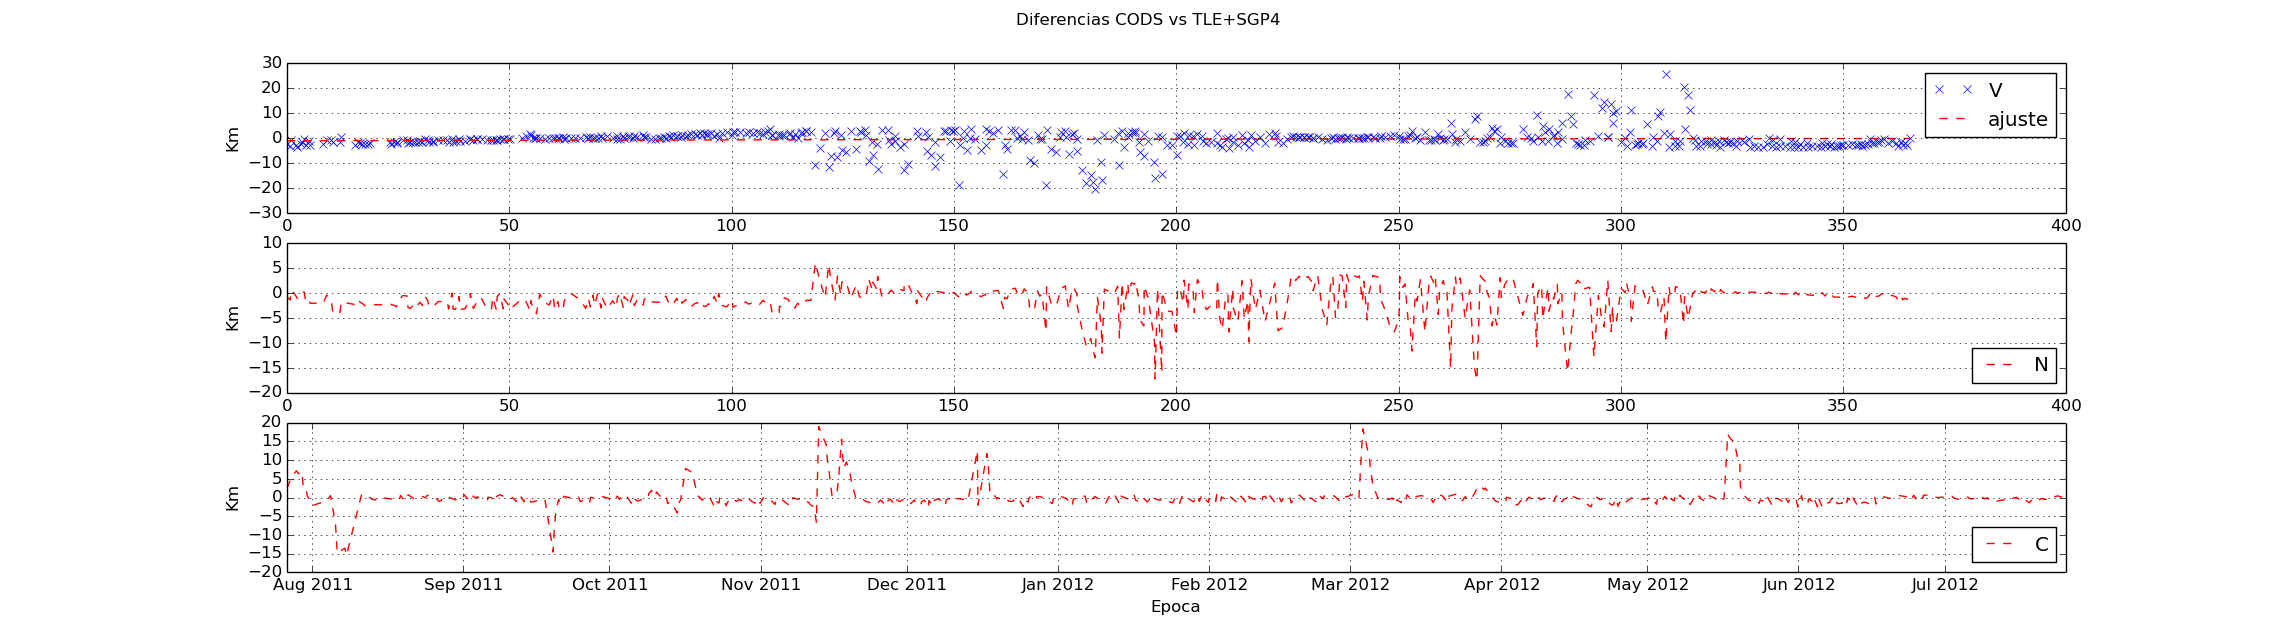
\includegraphics[width=\textwidth]{imagenes/sacDajusteG2}
\end{figure}
\begin{verbatim}
[ -9.98539126e-01   3.68651957e-03  -3.51802247e-06]
[array([ 10307.92893203]), 3, array([ 1.6541132 ,  0.5052889 ,  0.09269658])
1.2301271112846734e-13]
\end{verbatim}

\subsection{C\'ubico}
\begin{figure}[!h]
\centering
  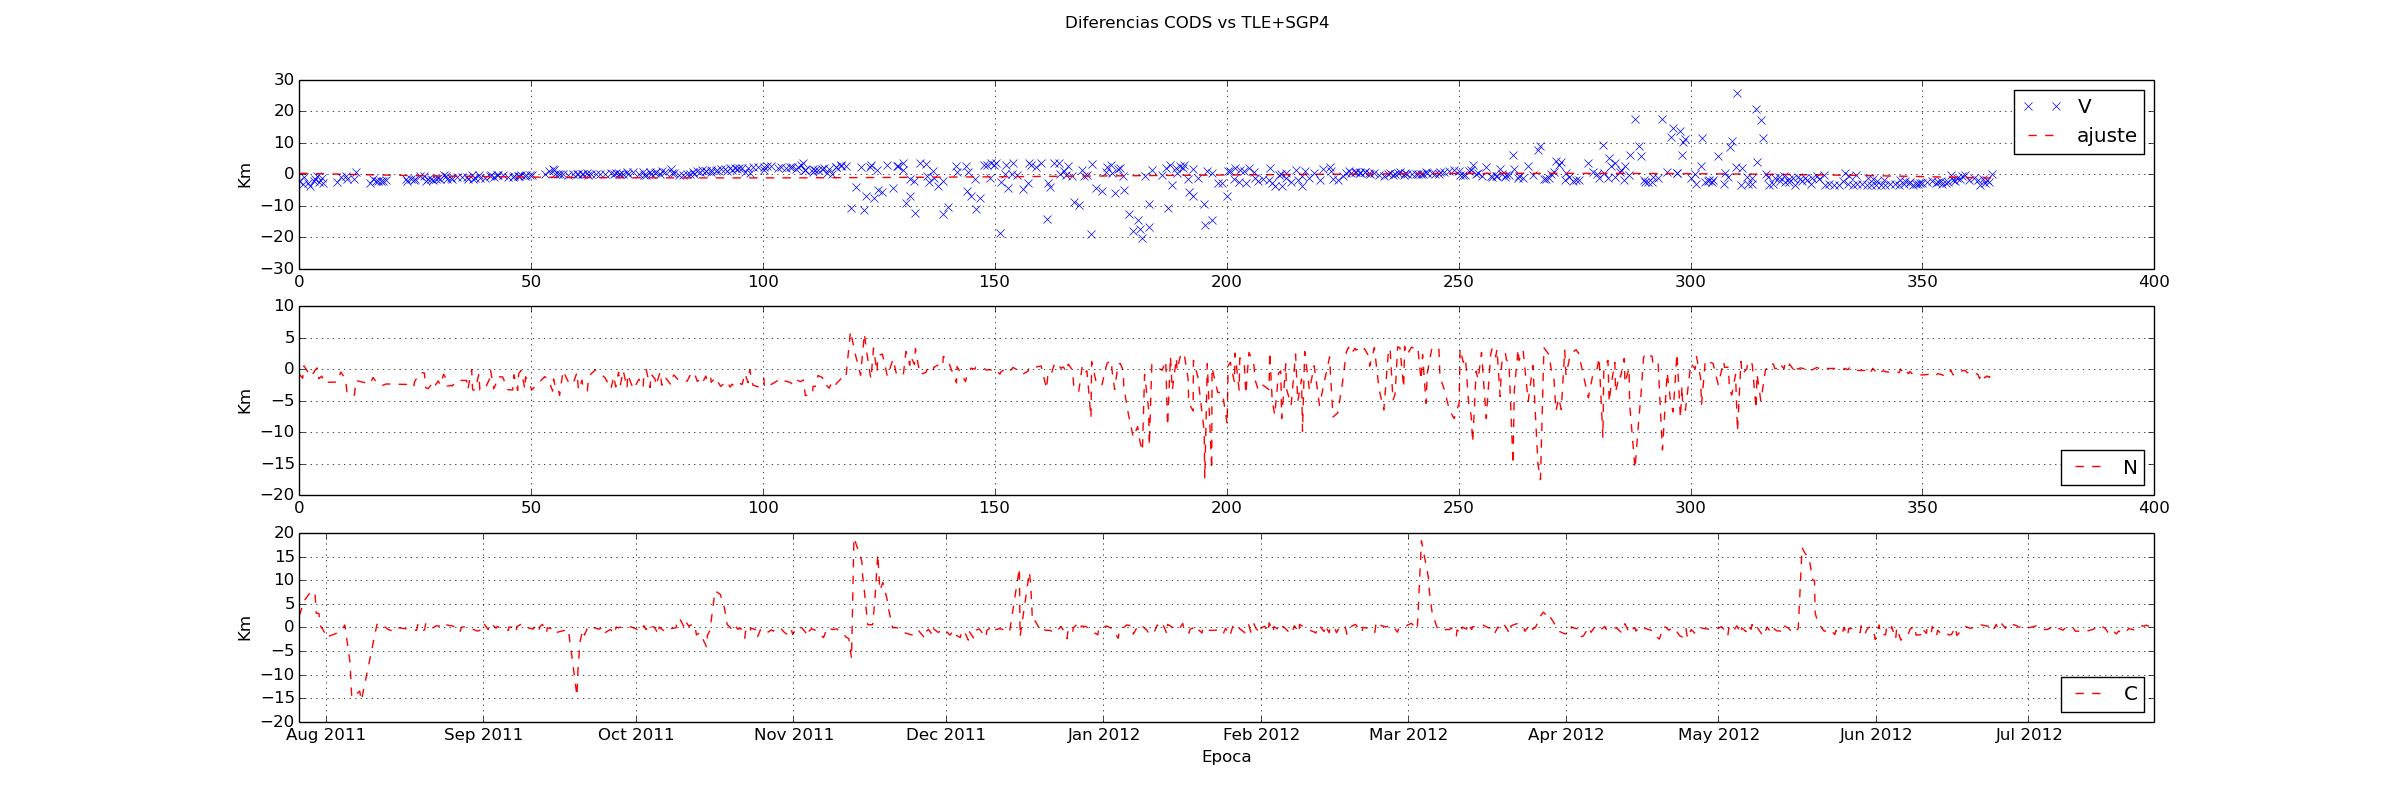
\includegraphics[width=\textwidth]{imagenes/sacDajusteG3}
\end{figure}
\begin{verbatim}
[  2.98290075e-01  -3.68802552e-02   2.69245141e-04  -4.92991794e-07]
[array([ 10194.70185149]), 4, array([ 1.89728074,  0.61374011,  0.15234123,  0.02100028])
1.2301271112846734e-13]
\end{verbatim}
